\section[Mitochondrial phylogenetic reconstruction]{Mitochondrial phylogenetic reconstruction - the power house of the phylogenies}
\label{cascade-sec:mitochondria}

While phylogenetic reconstruction is a well established method for genetic variants from canonical chromosomes to study metastatic progression and timing of evolutionary divergence \cite{Deshwar2015,Brown2017,Hu2019}, there are multiple issues. In \autoref{variantcalling-sec:phylo} and \autoref{variantcalling-sec:clonal} I showed how important the proper variant calling method is to accurately recover phylogenies and clonal patterns. 

However using somatic variants to reconstruct phylogenies is flawed to begin with, as most models studying genetic variation assume neutral evolution of the sites \cite{Kimura1968,Lynch1989}, but cancers almost exclusively exhibit positive selection \cite{Cannataro2018}. And while passenger mutations might not directly affect fitness of the cell, they only exist due to the link to the driver mutation and therefore has little to no additional information gain in addition to the driver. In addition, while in small populations genetic drift as a stochastic process overpowers selective processes (fitness coefficient $s$) and can therefore be assumed to be neutral, in larger populations $N_e$ (effective population size) where \autoref{mmf-eq:neutralSelection} does not hold true, mutations are under selective pressure \cite{EyreWalker2007}.
\begin{equation}
N_e \cdot s \ll 1 \label{mmf-eq:neutralSelection}
\end{equation}
\myequation[\ref{mmf-eq:neutralSelection}]{Selective pressure with effective population size}
%we need to squish this a bit otherwise it looks weird
\vspace{-3em}
All in all we can assume that with cancer growing, positive selection through treatment and tumour micro environmental niches, almost all assumptions of the coalescent theory are not applicable for tumour samples and therefore methods using somatic variants and their respective results need to be selected and evaluated carefully.

To tackle this issue, and assist with the interpretation of phylogenetic reconstruction results, we adjusted a method used in single cell sequencing to track clonal expansion with mitochondrial somatic mutations \cite{Ludwig2019} to be usable for standard bulk sequencing. Mitochondrial variants are an ideal source of clonality information, because the mutation rate is significantly higher than nuclear DNA, due to the missing proof reading and repair mechanisms, which allows very granular separation in a shorter time period. Additionally, while there are several diseases cause by defects in mitochondria such as Kearns-Sayre syndrom \cite{Harvey1992}, MERRF \cite{Adam1993} and MELAS \cite{Hirano1992}, they usually follow a mendelian inheritance pattern and are hereditary and not somatically acquired. In the cancer text, somatic mutations in mitochondrial DNA are assumed to be approximately neutral with a possible selection pressure towards healthy ageing and negatively selecting cancer \cite{Rodell2013,Yuan2020}.

\subsection{Method}
\label{cascade-sec:mitoMethod}

First a pileup of all mitochondrial positions is performed. Before the pileup we preselect reads which uniquely map to the mitochondrial genome and only retain high mapping quality reads. Then the nucleotide counts in each position is transformed into a MultiEssayExperiment \cite{Ramos2017} for final analysis in R. The preprocessing code and be found in \autoref{lst-cascadeAppendix:mitoPreProcessing}.

The final MultiEssayExperiment is then read into R and quality metrics applied to exclude samples with not enough coverage on the mitochondrial contig. usually WGS samples will show an extensive coverage of mitochondrial DNA, however WES will require a library preparation with probes in this area. Patient CA-I has a coverage of more than 100x for all but the germline sample which only has an overall coverage of 17x. Similar, patient CA-K \todo{add the stats}. All other Patients (CA-A/J/L) where samples are sequenced as WGS show a coverage of more than \todo{more stats}

\begin{figure}[!ht]
\centering
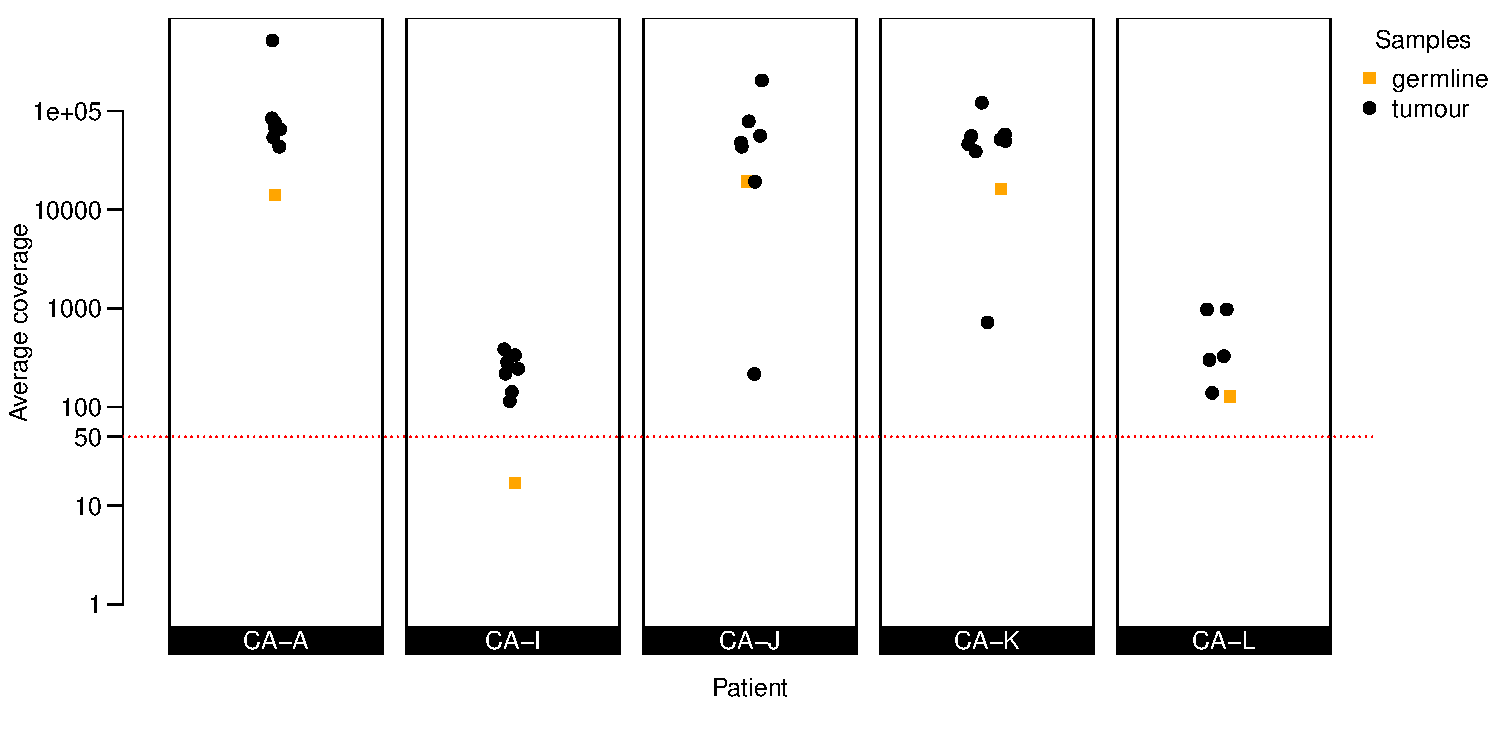
\includegraphics[width=.99\linewidth]{Figures/mtCoverage}
\vspace{-1em}
\caption[Average coverage of mitochondrial DNA of CASCADE patients]{Average coverage of mitochondrial DNA of CASCADE patients: Orange squares show germline sample for each patient; black points show tumour samples; horizontal red dotted line shows quality cut off suggested by \protect\textcite{Ludwig2019}} \label{fig:cas86schematic}
\end{figure}

To ensure optimal results, we will exclude all samples with an average coverage of less than 50x if it is a tumour sample and 15x for a germline sample. If only the tumour internal relations are of interest, the germline sample can also be removed from the analysis in case of lower coverage.
